\section{Estudio de los algoritmos de inteligencia artificial}

\label{cap4:analisisIA}

Los algoritmos Genético y de Recocido simulado son comparados aplicando pruebas en las mismas redes seleccionadas de la sección \ref{sec:cap4analisis}

En el caso del algoritmo genético también es mostrada la evolución de la función de evaluación.


\subsection{Red libre de escala}

\begin{figure}[H]
    \centering
    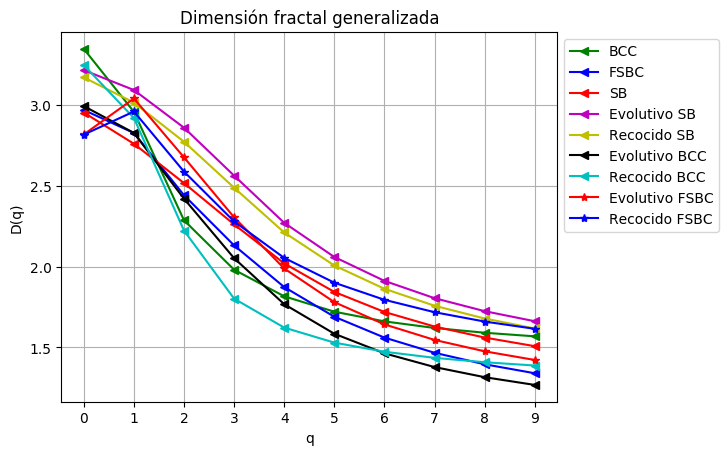
\includegraphics[scale=0.7]{{Capitulo4Multifractalidad/imagenesIA/grafica_Dq20180506_035455ScaleFree4000Nodes}.png}
    \caption{Multifractalidad en red libre de escala con 4000 nodos}
\end{figure}

\begin{figure}[H]
    \centering
    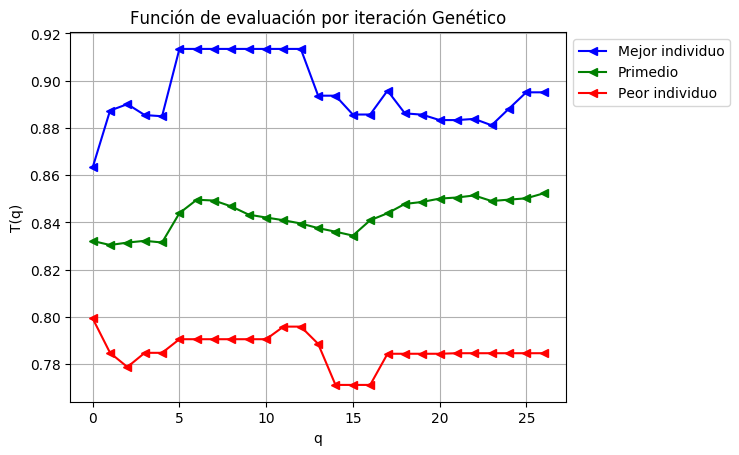
\includegraphics[scale=0.7]{{Capitulo4Multifractalidad/imagenesIA/grafica_Fitness20180502_203759ScaleFree2000Nodes.txt}.png}
    \caption{Evolución de la función de evaluación en red libre de escala con 4000 nodos}
\end{figure}

\subsection{Red de mundo pequeño}

\begin{figure}[H]
    \centering
    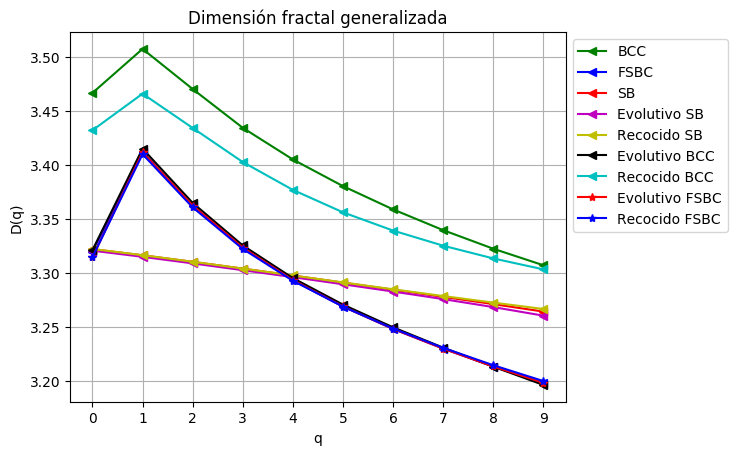
\includegraphics[scale=0.7]{{Capitulo4Multifractalidad/imagenesIA/grafica_Dq20180506_141058SmallWorld5000NodesRewire01.txt}.png}
    \caption{Multifractalidad en red de mundo pequeño de 5000 nodos con p = 10\%}
\end{figure}

\begin{figure}[H]
    \centering
    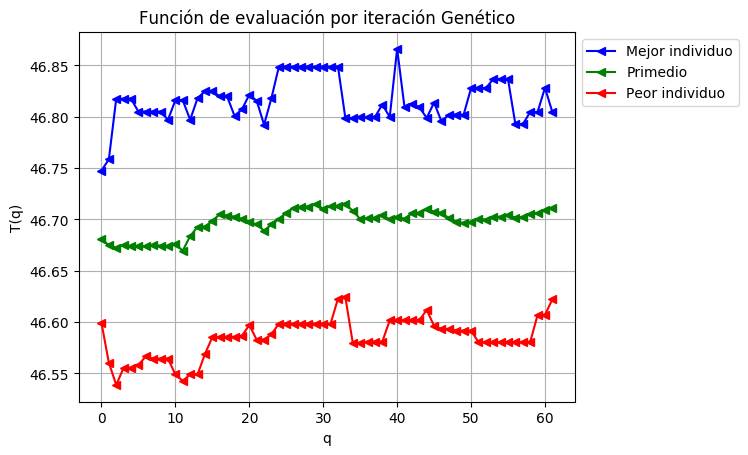
\includegraphics[scale=0.7]{{Capitulo4Multifractalidad/imagenesIA/grafica_Fitness20180506_141058SmallWorld5000NodesRewire01.txt}.png}
    \caption{Evolución de la función de evaluación en red de mundo pequeño de 5000 nodos con p = 10\%}
\end{figure}

\subsection{Red aleatoria}

\begin{figure}[H]
    \centering
    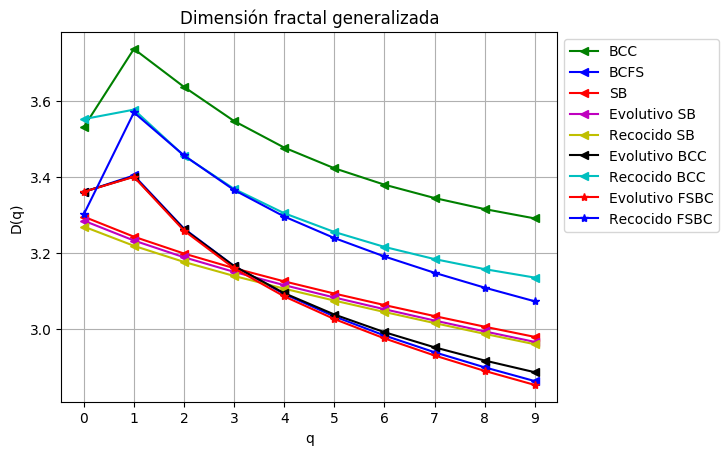
\includegraphics[scale=0.7]{{Capitulo4Multifractalidad/imagenesIA/grafica_Dq20180502_133953Random1991Nodes5939}.png}
    \caption{Multifractalidad en red aleatoria con 5620 nodos}
\end{figure}

\begin{figure}[H]
    \centering
    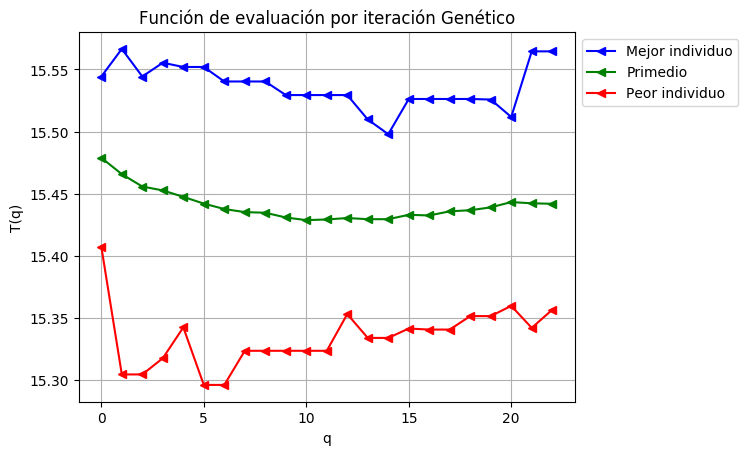
\includegraphics[scale=0.7]{{Capitulo4Multifractalidad/imagenesIA/grafica_Fitness20180508_231031Random3373Nodes5978.txt}.png}
    \caption{Evolución de la función de evaluación en red aleatoria con 5620 nodos}
\end{figure}

\subsection{Red observada bacteria Ecoli}

\begin{figure}[H]
    \centering
    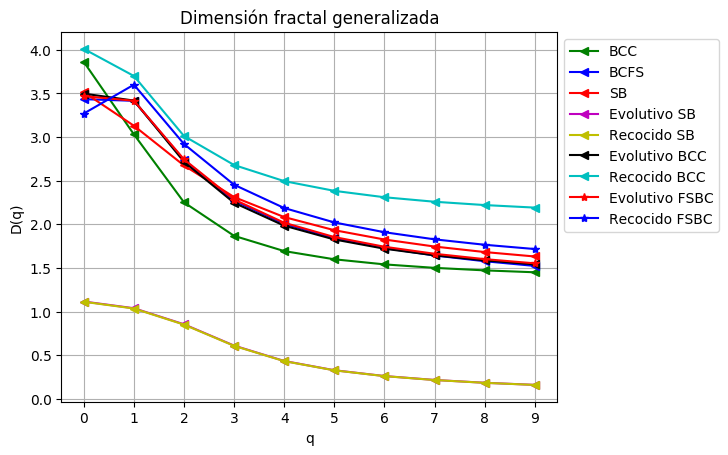
\includegraphics[scale=0.7]{{Capitulo4Multifractalidad/imagenesIA/grafica_Dq20180504_000006EColi}.png}
    \caption{Multifractalidad en red observada de Ecoli}
\end{figure}

\begin{figure}[H]
    \centering
    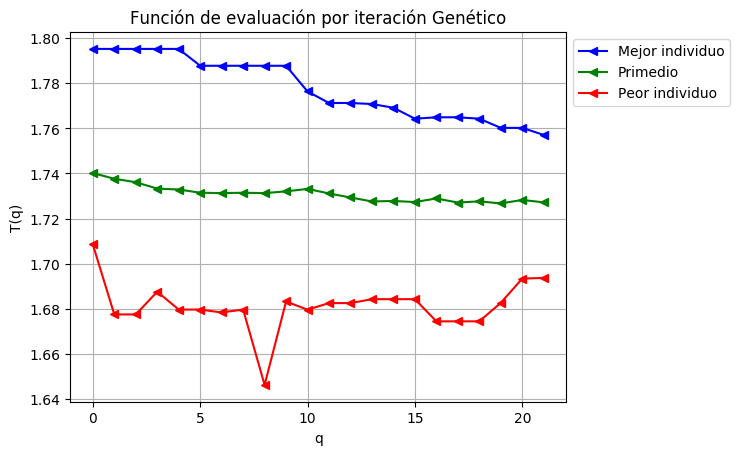
\includegraphics[scale=0.7]{{Capitulo4Multifractalidad/imagenesIA/grafica_Fitness20180508_182332cerevisiae.txt}.png}
    \caption{Evolución de la función de evaluación en red observada de Ecoli}
\end{figure}

\subsection{Red fractal}

\begin{figure}[H]
    \centering
    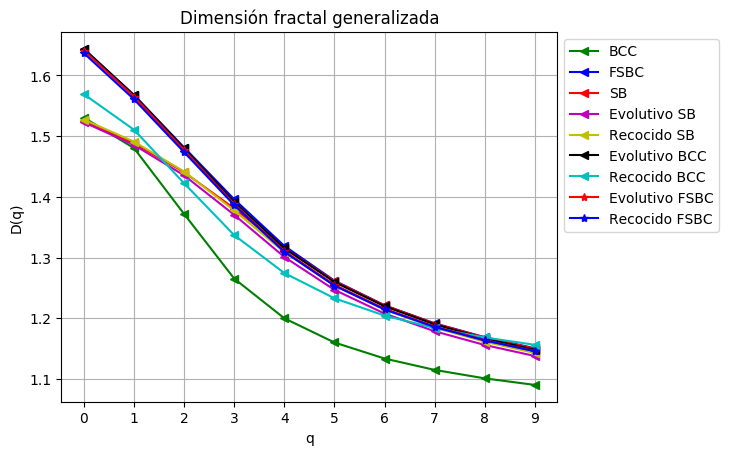
\includegraphics[scale=0.7]{{Capitulo4Multifractalidad/imagenesIA/grafica_Dq20180511_101739floweru2v2}.png}
    \caption{Multifractalidad en red generada fractal (2,2)-flower}
\end{figure}

\begin{figure}[H]
    \centering
    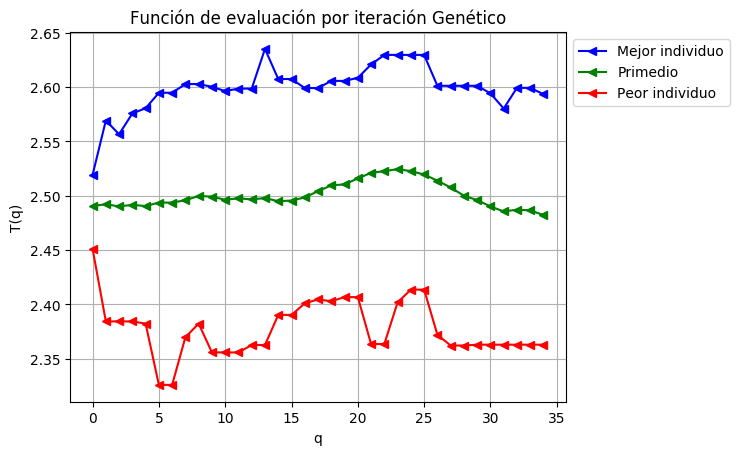
\includegraphics[scale=0.7]{{Capitulo4Multifractalidad/imagenesIA/grafica_Fitness20180511_101739floweru2v2.txt}.png}
    \caption{Evolución de la función de evaluación en red fractal (2,2)-flower}
\end{figure}

\subsection{Análisis de los algoritmos}

Se puede observar que:

\begin{enumerate}
    \item No es sencillo estimar un número de iteraciones para los algoritmos de inteligencia artificial, en algunos casos el resultados es muy cercano a los deterministas, en otros no.
    \item Dado que el tiempo requerido para la ejecución de los algoritmos es considerable (más de 100 horas) de acuerdo a tabla \ref{tab:executionTimes}, se requiere un soporte teórico para conocer el número de iteraciones óptimo para cada estrategia.
    \item Las gráficas de la evolución de la función de evaluación muestran que la heurística usada debe ser mejorada para validar cuales son los mejores centros. se observa una convergencia en las primeras generaciones.
\end{enumerate}

\section{Análisis de los tiempos de ejecución}

En la tabla \ref{tab:executionTimes} son analizados los tiempos de ejecución de cada uno de los algoritmos, de acuerdo al protocolo de pruebas especificado en el Anexo B de la página \pageref{AnexoB}

\begin{table}[H]
    \centering
    \begin{tabular}{|p{1cm}|p{1cm}|p{1.1cm}|p{1cm}|p{1.5cm}|p{1.5cm}|p{1.5cm}|p{1.5cm}|p{1.5cm}|p{1.5cm}|}
         \hline
         \textbf{Red} & \textbf{BCFS} & \textbf{BCC} & \textbf{SB} & \textbf{Genético BCFS} & \textbf{Recocido BCFS} &
         \textbf{Genético BCC} & \textbf{Recocido BCC} &
         \textbf{Genético SB} & \textbf{Recocido SB} \\
         \hline
         Red A & 10788 & 10715 & 1193 & 7097 & 5092 & 6324 & 4995 &4644 & 6653 \\
         \hline
         Red B & 84833 & 85043  & 16598  & 48511  & 38744  &  35022 & 48511 & 35067 & 48360  \\
         \hline
         Red C & 271062 & 380427 & 19535  &  16508 & 20410  &  27972 & 16508 & 24480 & 15692  \\
         \hline
         Red D & 106396 & 106751 &  60063 & 75580  & 61520  & 94662  & 57915  & 68997 &  60096 \\
         \hline
         Red E & 494803 & 394747 &  8430 & 13698  & 10614  & 31047  & 11136  & 14146 &  10448 \\
         \hline
    \end{tabular}
    \caption{Tiempos de ejecución para diferentes redes en segundos}
    \label{tab:executionTimes}
\end{table}

Se observa que en general los algoritmos BCFS y BCC tienen una mejora considerable cuando se les aplica estrategias de inteligencia artificial. Con respecto al algoritmo SB, se requiere realizar un estudio más amplio para llegar a una conclusión debido a que:

\begin{itemize}
    \item El número de iteraciones de SB depende del número de nodos y del número de repeticiones del algoritmo.
    \item El número de iteraciones de los algoritmos de IA depende los parámetros suministrados por el usuario.
\end{itemize}

Lamentablemente, los algoritmos requiere gran capacidad de cómputo y tiempo de ejecución, por lo que esto se debe realizar en un estudio posterior.